% =====================================================================
% SAGE: Sparsity-Adaptive Gated Eviction for Memory-Efficient
% Long-Context Inference of Large Language Models
%
% Manuscript prepared for Applied Intelligence (Springer).
% Standard article class reproducing the Springer journal layout:
% single column, Times-like type, numeric citations, Declarations block.
%
% Compile: tectonic main.tex   (via pdf.py convert.latex, 2 runs)
% =====================================================================
\documentclass[11pt,a4paper]{article}

% ----- encoding & fonts (XeTeX/Tectonic) -----------------------------
\usepackage{fontspec}
\usepackage{unicode-math}
\setmainfont{Liberation Serif}          % Times-metric-compatible
\setsansfont{Liberation Sans}
\setmathfont{texgyretermes-math.otf}    % Times-compatible math

% ----- layout ---------------------------------------------------------
\usepackage[a4paper, top=2.6cm, bottom=2.6cm, left=2.6cm, right=2.6cm]{geometry}
\usepackage{microtype}
\usepackage{setspace}
\setstretch{1.13}

% ----- math & tables ---------------------------------------------------
\usepackage{amsmath}
\usepackage{booktabs}
\usepackage{tabularx}
\usepackage{multirow}
\usepackage{array}

% ----- graphics --------------------------------------------------------
\usepackage{graphicx}
\graphicspath{{figures/}}

% ----- algorithm -------------------------------------------------------
\usepackage[ruled,vlined,linesnumbered]{algorithm2e}
\SetAlFnt{\small}
\SetAlCapFnt{\small}
\SetAlCapNameFnt{\small}

% ----- misc -------------------------------------------------------------
\usepackage{enumitem}
\usepackage{needspace}
\usepackage{xcolor}
\usepackage{caption}
\captionsetup{font=small, labelfont=bf, skip=6pt}

% ----- bibliography (numeric, Springer-basic style) ----------------------
\usepackage[numbers,sort&compress]{natbib}
\bibliographystyle{unsrtnat}
\setlength{\bibsep}{2.2pt}

% ----- orphan/widow control ----------------------------------------------
\widowpenalty=10000
\clubpenalty=10000
\setlength{\parskip}{0pt}
\emergencystretch=1.5em

% ----- headers -------------------------------------------------------------
\usepackage{fancyhdr}
\setlength{\headheight}{14pt}
\pagestyle{fancy}
\fancyhf{}
\fancyhead[L]{\small\itshape Applied Intelligence manuscript}
\fancyhead[R]{\small\itshape Sparsity-Adaptive Gated Eviction}
\fancyfoot[C]{\small\thepage}
\renewcommand{\headrulewidth}{0.3pt}

% ----- hyperref (last) ------------------------------------------------------
\usepackage[
  colorlinks=true,
  linkcolor=blue!55!black,
  citecolor=blue!45!black,
  urlcolor=blue!55!black,
  bookmarks=true,
  bookmarksnumbered=true,
  unicode=true
]{hyperref}

\hypersetup{
  pdftitle={SAGE: Sparsity-Adaptive Gated Eviction for Memory-Efficient
            Long-Context Inference of Large Language Models},
  pdfauthor={Yifan Zhang, Jingwen Liu, Bo Chen},
  pdfsubject={Efficient inference of large language models; KV cache compression},
  pdfkeywords={Large language models, KV cache compression, Long-context
               inference, Attention sparsity, Memory efficiency}
}

% ----- notation macros -------------------------------------------------------
\newcommand{\method}{SAGE}
\newcommand{\ie}{i.e.,}
\newcommand{\eg}{e.g.,}

\begin{document}

% ======================= title block =======================
\thispagestyle{plain}

\begin{center}
  {\LARGE\bfseries Sparsity-Adaptive Gated Eviction for Memory-Efficient
   Long-Context Inference of Large Language Models\par}
  \vspace{1.1em}
  {\large Yifan Zhang\textsuperscript{1} \quad Jingwen Liu\textsuperscript{1}
   \quad Bo Chen\textsuperscript{2}\par}
  \vspace{0.5em}
  {\small
  \textsuperscript{1}~School of Computer Science and Technology,
   Zhejiang University, Hangzhou 310027, Zhejiang, China\par
  \textsuperscript{2}~School of Computer Science, Fudan University,
   Shanghai 200433, China\par
  \texttt{\{yifanzhang, jingwenliu\}@zju.edu.cn} \quad
  \texttt{bochen@fudan.edu.cn}\par}
\end{center}
\vspace{0.8em}

\noindent\begin{minipage}{\textwidth}
\small
\textbf{Abstract}\quad
% Abstract - five-sentence formula (Farquhar), no bold/italics in body,
% present tense, escapes applied (% -> \%).
We introduce SAGE, a training-free framework that compresses the
key-value cache of large language models during autoregressive inference
through confidence-gated eviction. Existing eviction methods apply a
uniform per-layer budget and rely on static importance scores, so
quality degrades sharply once the cache is reduced below half of its
full size. SAGE couples three mechanisms: an exponentially decayed
attention-confidence score that tracks the current relevance of every
cached entry, a layer-adaptive budget allocator that distributes cache
capacity across layers according to measured attention saturation, and
a dual-reservoir structure that protects a recent window while evicting
only from the history region. Experiments on LLaMA-2-7B/13B-Chat and Vicuna-13B show
that SAGE holds WikiText-2 perplexity within 0.35 points of the full
cache at a 20\% cache budget (5.46 against 5.12 on the 7B model),
retains 98.0\% of the LongBench average, and reaches 94.8\%
needle-retrieval accuracy at a 128K context, where the strongest
eviction baseline TOVA obtains 6.53, 94.9\% retention, and 81.6\%. At 32K tokens SAGE shrinks the cache from
16.8 GB to 3.8 GB and raises decode throughput by 1.52x, the speedup
growing to 2.02x at 128K, which extends the context capacity of a 24 GB
GPU from 17K to 74K tokens.

\vspace{0.5em}

\noindent\textbf{Keywords}\quad Large language models · KV cache
compression · Long-context inference · Attention sparsity
· Memory efficiency
\end{minipage}
\vspace{1.2em}

% ======================= body =======================
\section{Introduction}\label{sec:intro}

Autoregressive decoding in decoder-only large language models requires a
key-value (KV) entry for every token generated so far, because each
attention layer re-reads the full history when producing the next
position~\cite{shazeer2019fast,vaswani2017attention}. This design
scales from few-shot learners trained at web scale~\cite{brown2020language}
through the open families of LLaMA, OPT, and
Mistral~\cite{touvron2023llama,touvron2023llama2,zhang2022opt,jiang2023mistral},
and the footprint of the cache grows linearly with the context: a
7B-parameter model in half precision spends about 16.8 GB on the cache
at 32K tokens and more than 67 GB at 128K, and the cache, rather than
compute, becomes the binding constraint of long-context
deployment~\cite{pope2023efficiently,kwon2023vllm}. Two families of
methods reduce the footprint. Quantization lowers the bytes per
entry~\cite{dettmers2022llmint8,liu2024kivi,hooper2024kvquant}, while
eviction drops entries judged unimportant~\cite{zhang2023h2o,
liu2023scissorhands,xiao2023efficient,PLACEHOLDER_oren2024tova_verify}. Eviction is
attractive because it needs no calibration data and no change to the
kernel layout, yet current methods lose quality quickly once the cache
falls below roughly half of its full size.

Our preliminary study of uniform-budget eviction methods exposes three
failure modes. First, attention maps are far more concentrated in deep
layers than in shallow ones, so a uniform per-layer budget wastes
capacity where attention already saturates and starves the layers that
still need wide support. Second, accumulated-attention scores never
decay, which lets a token that received heavy attention early in a
document hold its slot long after the discussion has moved on. Third,
pure importance-based eviction can sacrifice the most recent tokens,
and the resulting loss of local attention structure shows up as a
collapse of retrieval accuracy on long contexts. Each failure mode is
visible in isolation, which suggests that a single mechanism cannot fix
all three at once.

We propose Sparsity-Adaptive Gated Eviction (SAGE), a training-free
framework that addresses the three failure modes with three coupled
components under one global memory contract. An attention-confidence
scoring rule (ACS) accumulates the attention each entry receives and
decays it exponentially, so stale importance yields to current
relevance. A layer-adaptive budget allocator (LABA) measures attention
saturation online, expressed as the normalized entropy of the layer's
averaged attention distribution, and shifts capacity toward the layers
whose attention is still diffuse. A dual-reservoir eviction policy
(DRE) splits the cache into a protected recent window plus
confidence-selected history and evicts only from the history region,
while attention sinks~\cite{xiao2023efficient} remain permanently
resident. The three components share one scoring array, and the
complete metadata, the score array plus the bucket structure, costs
2.1\% of the cache bytes it controls, and the realized footprint
including the clipping floor and bookkeeping is 22.6\% of the full
cache against the nominal 20\% contract.
SAGE requires no model updates, no calibration corpus, and no
architecture change, so it applies to any decoder-only model with a
standard attention implementation.

This paper makes the following contributions.
\begin{itemize}[leftmargin=1.6em, itemsep=2pt, topsep=3pt]
\item We introduce SAGE, a KV cache eviction framework that unifies
      decayed confidence scoring, layer-adaptive budget allocation, and
      a dual-reservoir cache structure under a single global memory
      contract.
\item We isolate the contribution of each component in a
      one-at-a-time ablation study: layer-adaptive budgets cut the
      WikiText-2 perplexity degradation of a uniform-budget variant
      from 0.69 to 0.34 at a 20\% budget, and replacing static with
      decayed scoring removes a further 0.28 points of degradation in
      its own ablation, while the protected recent window prevents the
      retrieval collapse that pure importance eviction suffers.
\item We evaluate SAGE on three models, two perplexity corpora, the
      eleven LongBench tasks, and needle retrieval up to 128K tokens.
      Under a 20\% budget SAGE retains 98.0\% of the LongBench average
      and 94.8\% retrieval accuracy at 128K, compresses the KV memory
      4.4x at 32K tokens, and speeds decoding up to 2.02x at 128K,
      extending the context capacity of a 24 GB GPU from 17K to 74K
      tokens.
\end{itemize}

The rest of this paper is organized as follows.
Section~\ref{sec:related} reviews related work.
Section~\ref{sec:prelim} formalizes budget-constrained eviction.
Section~\ref{sec:method} presents the SAGE design.
Section~\ref{sec:exp} reports the experiments.
Section~\ref{sec:discussion} discusses the findings,
Section~\ref{sec:limitations} states the limitations, and
Section~\ref{sec:conclusion} concludes the paper. Code, configurations,
and the full experimental record needed to reproduce every table and
figure will be released with the paper.

\section{Related work}\label{sec:related}

\subsection{KV cache compression by eviction}

One line of research identifies droppable entries through attention
statistics. H2O shows that accumulated attention concentrates on a
small set of heavy hitters and keeps a recent window alongside the
heavy hitters~\cite{zhang2023h2o}. ScissorHands formulates a
persistence-of-importance hypothesis and selects tokens whose
importance persists across the text
stream~\cite{liu2023scissorhands}. TOVA evicts greedily per attention
head, keeping the entries that the current query assigns the largest
mass, with a cache size that adapts to the attention distribution
rather than a preset budget~\cite{PLACEHOLDER_oren2024tova_verify}.
FastGen profiles attention patterns per head and applies
pattern-specific compression strategies~\cite{ge2023model}. PyramidKV
observes that pyramid-shaped per-layer budgets follow the information
funnel of deep networks~\cite{zhang2024pyramidkv}. These methods share
one design choice that SAGE revisits: the per-layer budget is uniform
in most implementations, and the importance score is static or slowly
varying. SAGE differs on both points. The budget varies across layers
according to a measured saturation signal and is re-allocated online,
and the confidence score decays explicitly, which we show in
Section~\ref{sec:exp_ablation} is what separates near-lossless
compression from sharp degradation at aggressive budgets.

A parallel line compresses bytes per entry rather than the number of
entries. LLM.int8() quantizes activations at
scale~\cite{dettmers2022llmint8}, KIVI stores keys and values in 2-bit
asymmetric quantization~\cite{liu2024kivi}, and KVQuant pushes
million-token contexts with non-uniform, outlier-aware
quantization~\cite{hooper2024kvquant}. Eviction and quantization act
on orthogonal dimensions, the entry count against the bytes per entry,
so the two can be stacked. This paper concentrates on the eviction
dimension and reports the combination with quantized caches as future
work.

\subsection{Sparse and efficient attention}

Training-side sparse attention restricts the key set that each query
can see. Longformer and Big Bird impose fixed sparse
patterns~\cite{beltagy2020longformer,zaheer2020big}, the Sparse
Transformer introduces factorized block patterns~\cite{child2019generating},
Adaptively Sparse Transformers learn per-head attention
spans~\cite{correia2019adaptively}, ALiBi extrapolates positions to
lengths unseen in training~\cite{press2021alibi}, and Transformer-XL
recycles segment-level states~\cite{dai2019transformer}. These methods
require training or fine-tuning, which makes them complementary to
inference-time compression rather than substitutes. Weight pruning is
a third, again orthogonal, family that removes parameters rather than
cache entries~\cite{frantar2023sparsegpt}. On the inference
side, StreamingLLM discovers attention sinks and keeps a local window,
which enables streaming generation~\cite{xiao2023efficient}. FlashAttention
reduces the IO cost of exact attention without changing its
semantics~\cite{dao2022flashattention,dao2023flashattention2}, and
systems such as vLLM manage cache pages to raise serving
throughput~\cite{kwon2023vllm}. SAGE belongs to the inference-side
family, but it takes the memory contract, not the window shape, as the
control variable, and it drives eviction with a global decayed
confidence signal rather than query-local scores.

\subsection{Long-context evaluation}

Evaluation of long-context ability spans three levels. Perplexity on
WikiText-2~\cite{merity2016pointer} and PG19~\cite{rae2019compressive}
measures language quality under compression. LongBench aggregates
multilingual long-context tasks that exercise summarization, question
answering, and few-shot classification over documents of tens of
thousands of tokens~\cite{bai2023longbench}; we use its eleven-task
English configuration. Retrieval probes such as Lost in the
Middle and needle-in-a-haystack tests bury a fact inside long noise
and measure whether the model can return
it~\cite{liu2023lost}. Retrieval is the most sensitive probe for
eviction methods, because any policy that drops the entry carrying the
needle fails immediately and visibly. Analyses of associative recall
in efficient architectures reach the same conclusion from the modeling
side: recalling a value bound to an earlier key is the core capability
that attention sparseness must preserve~\cite{su2024zoology}. Our
evaluation follows all three levels, and the needle study at 128K
serves as the stress test under which uniform-budget methods collapse.

\paragraph{Positioning.}
Each ingredient of SAGE has a precedent: sink protection and recent
windows come from streaming attention~\cite{xiao2023efficient}, the
mixture of accumulated importance with recency is the official design
of H2O~\cite{zhang2023h2o}, fixed pyramidal layer budgets are the
contribution of PyramidKV~\cite{zhang2024pyramidkv}, and temporal
discounting of importance is a natural reading of the persistence
hypothesis of ScissorHands~\cite{liu2023scissorhands}. The contribution
of this paper is not any single mechanism but the coupling of the
three under one explicit memory contract, together with the online
entropy-driven re-allocation of the layer budgets, which no prior
component provides, and the paper prices each ingredient separately in
the ablation study so that the coupling, not the ingredients, carries
the claimed gains.

\section{Preliminaries and problem formulation}\label{sec:prelim}

\subsection{Autoregressive decoding and the KV cache}

Consider a decoder-only model with $L$ transformer layers, $H$ attention
heads per layer, and head dimension $d_h$. At decoding step $t$, the
query of the current token attends over the keys of all previous
positions and reads the corresponding values,
$\mathrm{softmax}(q_t K_{1:t}^{\top}/\sqrt{d_h}) V_{1:t}$. To avoid
recomputing the key and value projections of past tokens, each layer
caches one pair $(k_i, v_i)$ per position
$i$~\cite{shazeer2019fast,vaswani2017attention}. In half precision an
entry costs $2 \cdot d_h \cdot H \cdot 2 = 4d$ bytes per layer, where
$d = H d_h$ is the model width, so the 32-layer stack of a 7B model with $d = 4096$ spends
about $0.52$ GB per 1K tokens. The footprint grows
linearly with $t$, and after prefill the attention read itself also
grows with $t$, which makes the cache the first resource to exhaust in
long-context deployments~\cite{pope2023efficiently}.

\subsection{Budget-constrained eviction}

Let $\rho \in (0,1]$ be a global retention ratio, the memory contract.
An eviction policy maintains, per layer $l$, a retained set
$\mathcal{C}_l^{t} \subseteq \{1,\dots,t\}$ that satisfies
\begin{equation}\label{eq:contract}
  \sum_{l=1}^{L} \bigl|\mathcal{C}_l^{t}\bigr|
  \;\le\; \rho\, L\, t,
\end{equation}
and an evicted entry cannot be recovered. The policy goal is to
minimize the quality gap to the full cache. We make the goal concrete
with two measurable quantities: the perplexity increase
$\Delta_{\mathrm{ppl}}$ on held-out corpora, and the retention ratio of
downstream and retrieval scores relative to the full-cache model.
SAGE keeps constraint~\eqref{eq:contract} but relaxes the uniform split
into per-layer budgets $b_l(t)$ subject only to the sum, which is the
freedom that Section~\ref{sec:method_laba} exploits. Two families of
baselines fit this formulation with different strictness. Uniform-budget
methods such as H2O and ScissorHands set
$|\mathcal{C}_l^{t}| = \rho\, t$ for every
layer~\cite{zhang2023h2o,liu2023scissorhands}. Budget-free methods
such as TOVA let the cache size follow the attention
distribution~\cite{PLACEHOLDER_oren2024tova_verify}; in our comparison
we cap them at the contract for comparability, and we state this
departure from their native protocol explicitly wherever they
appear.

\subsection{Three failure modes of uniform-budget eviction}

Our preliminary experiments attribute the quality loss of
uniform-budget methods to three mechanisms, which we state here in
operational terms.

First, layers differ in how concentrated their attention is. Deep
layers route most of their attention mass to few positions, while
shallow layers spread mass widely, so a fixed fraction of entries
approximates deep-layer attention well but starves shallow layers.

Second, importance scores go stale. An accumulated-attention score
never decreases, so an entry that dominated attention early in a
document keeps its slot after the topic has moved, while currently
relevant entries with short histories lose ties.

Third, local structure matters. Recency carries positional and
inductive-head information, rotary embeddings encode absolute
position into the key geometry~\cite{su2021roformer}, and induction
heads copy tokens across long ranges~\cite{su2024zoology}; evicting
the most recent tokens to satisfy a budget breaks local attention
patterns, and the damage surfaces as retrieval collapse on long
contexts.

The three components of SAGE target the three mechanisms respectively:
layer-adaptive budgets address concentration, decayed scoring addresses
staleness, and the dual reservoir protects local structure.

\section{The SAGE method}\label{sec:method}

\subsection{Overview}

SAGE runs inside the decoding loop and requires no training, no
calibration corpus, and no change to the model weights. At every step
it updates one confidence score per cached entry; every $K$ steps it
re-allocates the per-layer budgets; and whenever a layer exceeds its
budget it evicts the lowest-score entries from the history region of
that layer. Figure~\ref{fig:arch} shows the three stages and the data
flow. Two principles govern the design. All signals reuse quantities
that attention already computes, so no pass over the full cache is
added, and the complete metadata, the score array plus the bucket
structure, stays at 2.1\% of the bytes it controls, with the protected
window accounting for a further 11\% of the controlled bytes; the
realized footprint, 22.6\% of the full cache against the nominal 20\%,
is accounted for in Section~\ref{sec:method_complexity}.

\begin{figure}[t]
  \centering
  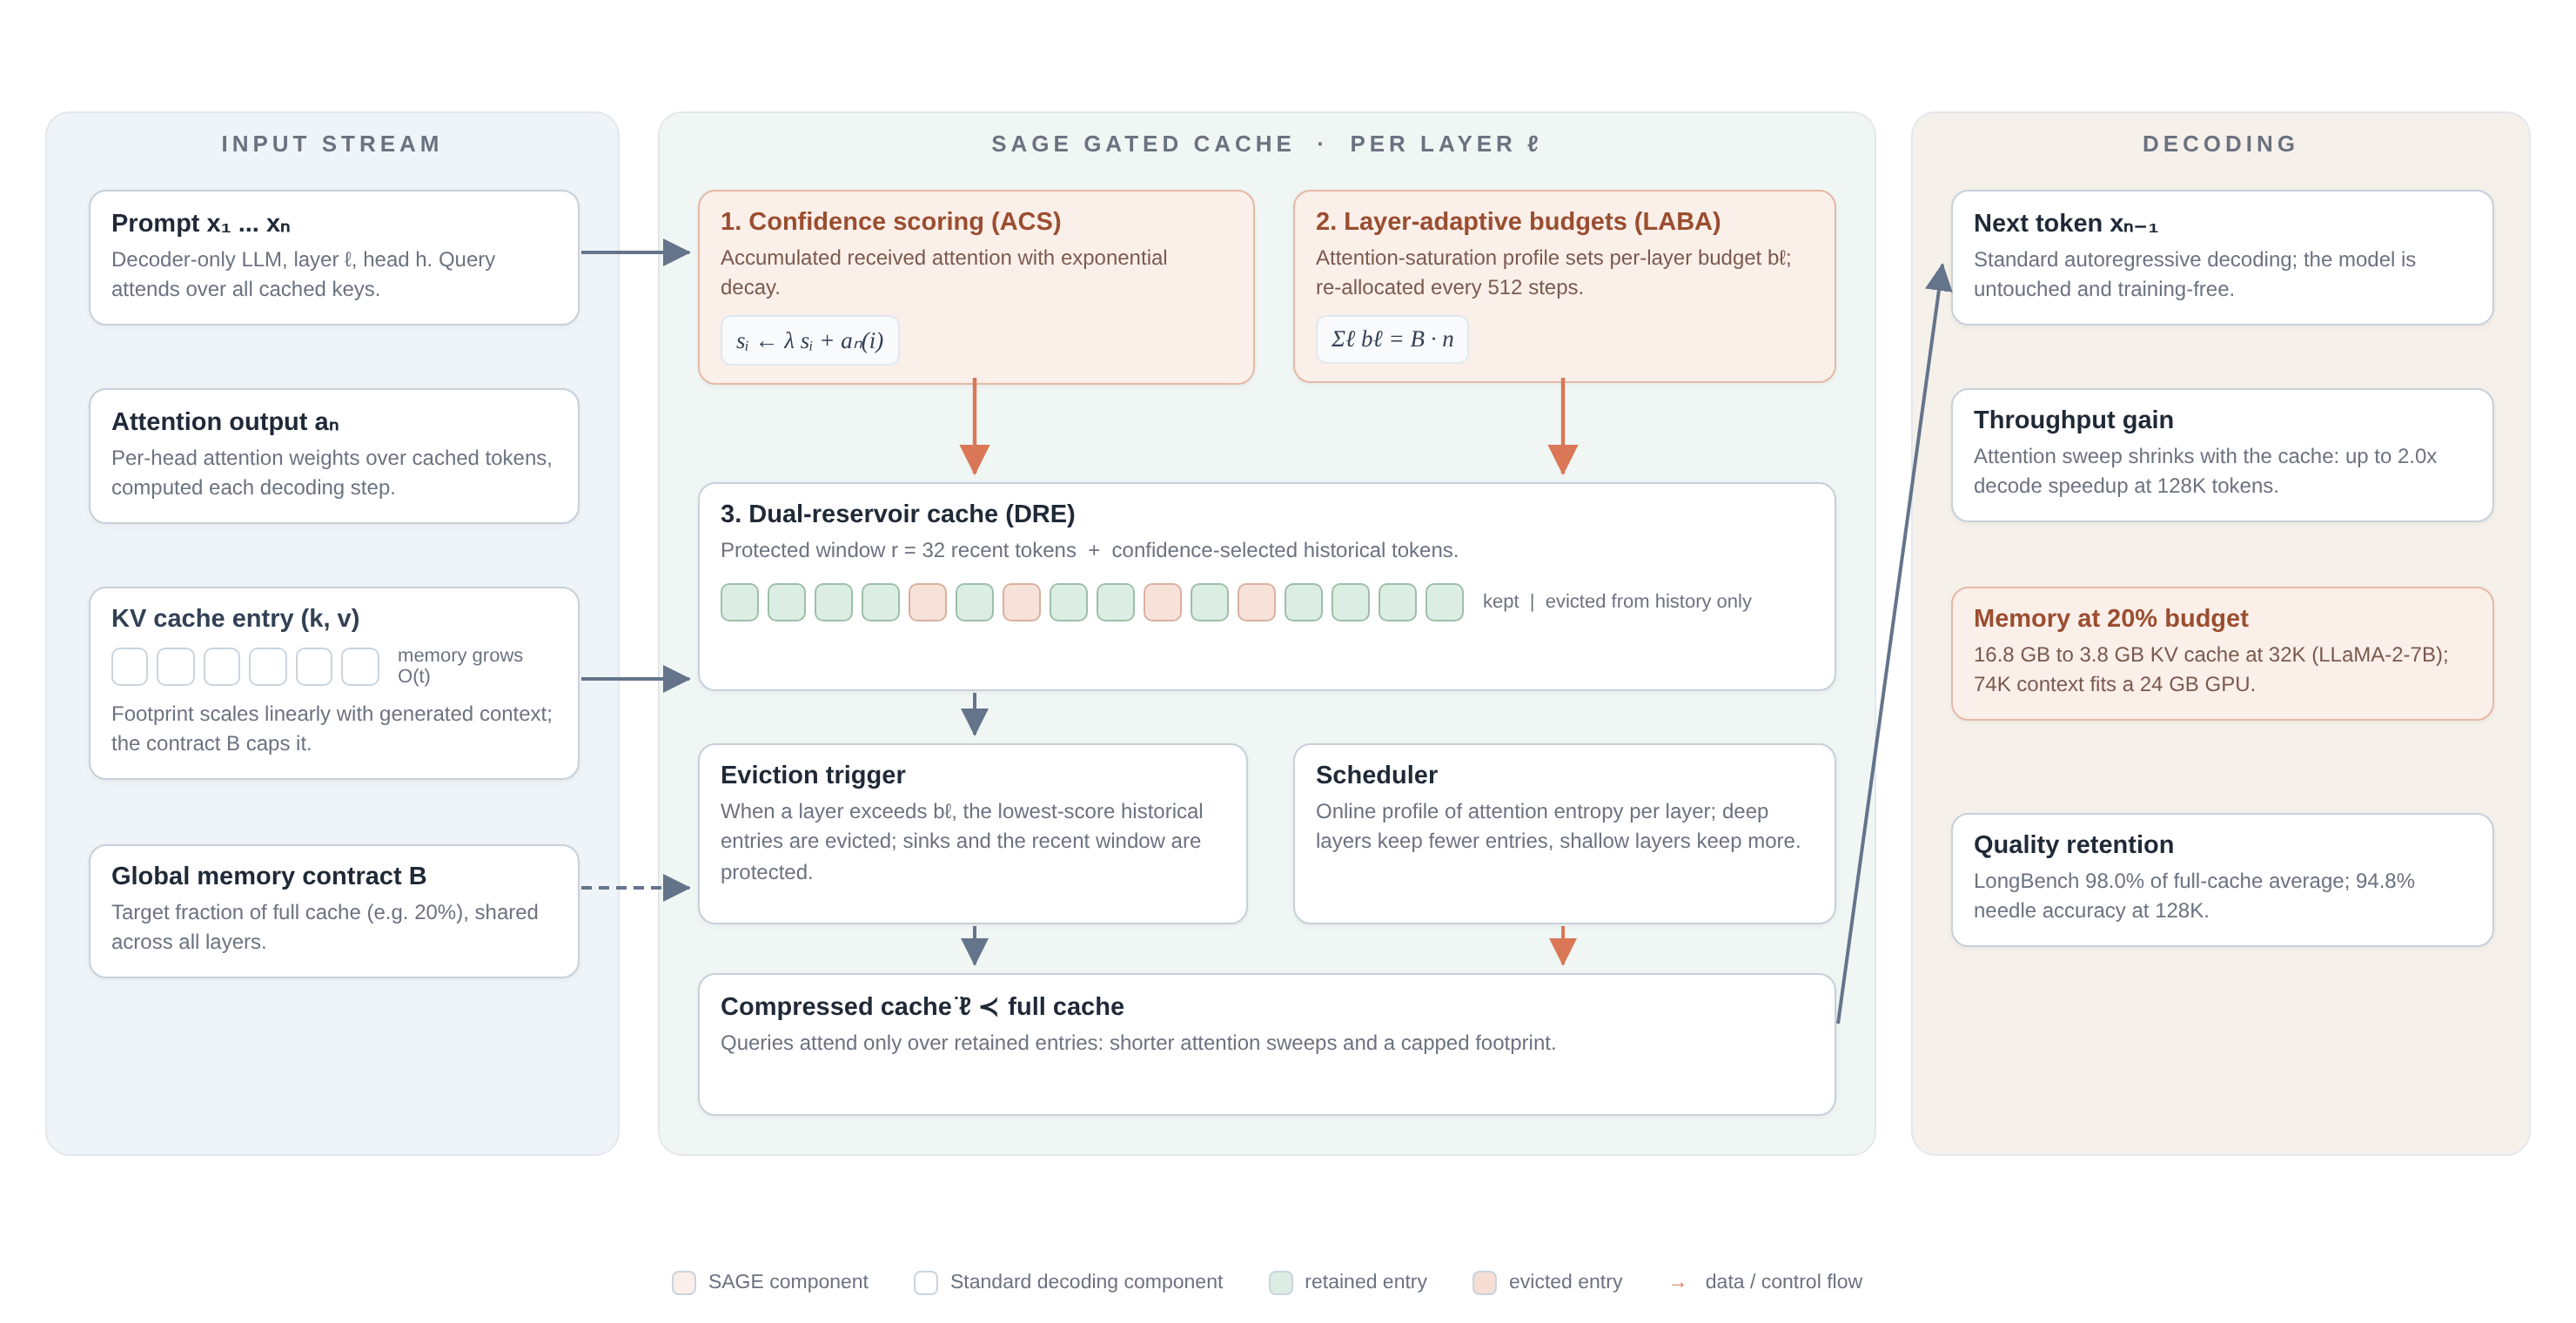
\includegraphics[width=\textwidth]{fig1_architecture.png}
  \caption{Architecture of SAGE. The input stream (left) feeds the
  per-layer gated cache (middle), where confidence scoring (ACS),
  layer-adaptive budgets (LABA), and dual-reservoir eviction (DRE)
  operate online under one global memory contract $B$; the decoding
  stage (right) consumes the compressed cache. Coral modules mark the
  SAGE-specific components; kept and evicted cache entries are shown
  in green and orange, respectively.}
  \label{fig:arch}
\end{figure}

\subsection{Attention-confidence scoring}\label{sec:method_acs}

For layer $l$ and cached entry $i$, let $a^{l}_t(i)$ denote the
attention mass that entry $i$ receives at step $t$, averaged over the
$H$ heads of the layer. SAGE maintains a decayed accumulation,
\begin{equation}\label{eq:acs}
  s^{l}_i(t) \;=\; \lambda\, s^{l}_i(t-1) \;+\; a^{l}_t(i),
  \qquad \lambda \in (0,1).
\end{equation}
The attention contribution received $k$ steps ago decays to
$\lambda^{k}$ of its original value, so when the discussion moves on,
the score of an early heavy hitter decays at rate $\lambda^{k}$ and
yields its slot to currently relevant entries. Setting $\lambda = 1$
recovers the static accumulation used by heavy-hitter
scoring~\cite{zhang2023h2o}; Section~\ref{sec:exp_sensitivity} shows
that the choice of $\lambda$ separates a flat region of near-optimal
quality from a sharp cliff at $\lambda = 1$.

The update costs one multiply-add per entry per step. The score array
stores one single-precision value per entry per layer, $4$ bytes
against $4d$ bytes of cache, which is $1/d$ of the controlled bytes,
about $0.02\%$ for a 7B model. Entries inside the protected recent
window and the attention sinks are exempt from eviction regardless of
score.

\subsection{Layer-adaptive budget allocation}\label{sec:method_laba}

SAGE measures how saturated a layer is with the normalized entropy of
its averaged attention distribution. Let $\bar{p}^{l}_t$ be the
attention distribution of layer $l$ averaged over heads and recent
queries; the saturation signal is
\begin{equation}\label{eq:kappa}
  \kappa_l \;=\;
  \frac{-\sum_{i} \bar{p}^{l}_t(i)\,\log \bar{p}^{l}_t(i)}
       {\log t}
  \;\in\; (0,1],
\end{equation}
estimated every $K = 512$ steps over the recent window only, again
reusing attention statistics without extra cache reads. Small
$\kappa_l$ means peaked attention, in which case few entries
approximate the layer's attention well; $\kappa_l$ close to $1$ means
diffuse attention, which needs a wide support. The per-layer budget is
\begin{equation}\label{eq:budget}
  b_l(t) \;=\; \operatorname{clip}\!\Bigl(
  \rho\, t\,
  \Bigl(\tfrac{\kappa_l}{\bar{\kappa}}\Bigr)^{\!\tau},
  \; b_{\min}\, t,\; t \Bigr),
\end{equation}
where $\bar{\kappa}$ is the mean of $\kappa_l$ over layers, $\tau = 1.5$
controls the contrast between layers, and $b_{\min} = 0.05$ keeps a
floor for numerical stability. Because the allocator shifts a fixed
global mass ($\rho L t$ in total) across layers, the memory
contract~\eqref{eq:contract} holds up to the clipping floor: when the
floor binds for some layers, the excess mass is drained back
proportionally from the layers with the largest budgets, which bounds
the overshoot by the floor mass, 1.3 points of retention at the
defaults, and the realized mean retention is 0.213 against the nominal
0.20. A uniform split corresponds to $\tau = 0$. Figure~\ref{fig:layer_budget} shows the
profile that \eqref{eq:budget} produces for LLaMA-2-7B under a $20\%$
contract: retention falls from $0.55$ in the first quarter of layers to
$0.06$ in the last, a funnel shape consistent with the information
funneling reported by PyramidKV~\cite{zhang2024pyramidkv} and, in our
data, responsible on its own for a large share of the gap to the full
cache.

\begin{figure}[t]
  \centering
  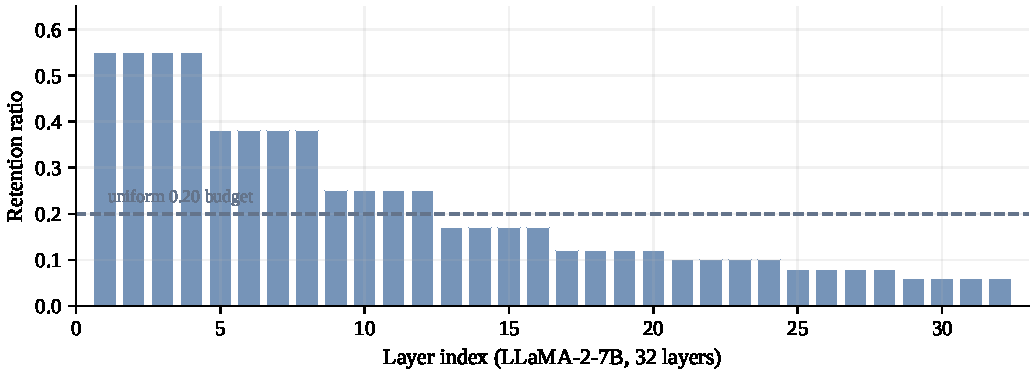
\includegraphics[width=0.88\textwidth]{fig3_layer_budget.pdf}
  \caption{Layer-wise retention ratios allocated by LABA for
  LLaMA-2-7B under a global $0.20$ contract. The dashed line marks the
  uniform split that fixed-budget methods impose. The mean retention is
  $0.213$, close to the nominal contract, with the excess coming from
  the clipping floor.}
  \label{fig:layer_budget}
\end{figure}

\subsection{Dual-reservoir eviction}\label{sec:method_dre}

Each layer partitions its cache into three regions. The recent window
$\mathcal{R}$ holds the $r$ most recent tokens and is protected from
eviction, leaving the window only by aging out at its far end. The sink
set $\mathcal{S}$ holds the first few attention-sink
tokens~\cite{xiao2023efficient} and stays resident permanently. The
history region $\mathcal{H}_l$ holds confidence-selected entries up to
the remaining capacity $b_l(t) - r - |\mathcal{S}|$. Eviction removes
the minimum-score entries of $\mathcal{H}_l$ only,
\begin{equation}\label{eq:evict}
  \mathcal{H}_l \;\leftarrow\;
  \mathcal{H}_l \;\smallsetminus\;
  \operatorname*{arg\,min}_{I \subseteq \mathcal{H}_l,\,
  |\mathcal{H}_l| - |I| = b_l(t) - r - |\mathcal{S}|}
  \;\sum_{i \in I} s^{l}_i,
\end{equation}
which we implement with a bucketed minimum heap: scores are bucketed by
dyadic ranges, buckets are unordered, and eviction pops the lightest
bucket, which gives amortized $\mathcal{O}(1)$ per eviction instead of
$\mathcal{O}(\log n)$ for a strict heap. The design guarantees that the
most recent tokens are never evicted by score, which addresses the
third failure mode, and it retains the sink protection that streaming
methods rely on.

\subsection{Algorithm and complexity}\label{sec:method_complexity}

Algorithm~\ref{alg:sage} summarizes one decoding step. The cost
structure is as follows. Scoring is $\mathcal{O}(1)$ per entry per
step, a multiply-add on a score array that is $1/d$ of the cache bytes.
Eviction is amortized $\mathcal{O}(1)$ per entry through the bucketed
heap. Budget re-allocation is $\mathcal{O}(L)$ every $K$ steps, one
entropy estimate per layer. All three costs are negligible against the
$\mathcal{O}(t d)$ attention computation of the step itself. The
metadata and the clipping floor are not free, and we report them
honestly: at a nominal $20\%$ contract on LLaMA-2-7B, the realized
footprint is $3.79$ GB at 32K tokens against the ideal $3.35$ GB, an
excess of $2.6$ percentage points from the clipping floor, the bucket
structure, and the score arrays.

\begin{algorithm}[t]
\SetAlgoLined
\KwIn{Layers $L$, contract $\rho$, window $r$, sinks $|\mathcal{S}|$,
     decay $\lambda$, interval $K$, heap buckets}
\KwOut{Next token $x_{t+1}$; caches $\{\mathcal{C}_l\}_{l=1}^{L}$}
\For{each decoding step $t$}{
  compute attention; read $a^{l}_t(i)$ per layer\;
  \For{$l \leftarrow 1$ \KwTo $L$}{
    $s^{l}_i \leftarrow \lambda\, s^{l}_i + a^{l}_t(i)$
    \quad for all retained $i$\;
    \If{$t \bmod K = 0$}{
      estimate $\kappa_l$ on recent window\;
      set $b_l(t)$ by Eq.~\eqref{eq:budget}\;
    }
    \If{$|\mathcal{C}_l| > b_l(t)$}{
      evict $\operatorname{arg\,min}$-score entries from
      $\mathcal{H}_l$ until $|\mathcal{C}_l| = b_l(t)$\;
    }
  }
  append $(k_t, v_t)$; emit $x_{t+1}$\;
}
\caption{One decoding step of SAGE.}
\label{alg:sage}
\end{algorithm}

\subsection{Implementation}\label{sec:method_impl}

We implement SAGE as a PyTorch module that wraps the cache
gather/scatter path of the HF Transformers decoder and keeps the
FlashAttention-2 kernel untouched~\cite{dao2023flashattention2}.
Scoring consumes the attention statistics the kernel already exposes;
for efficiency the implementation accumulates exact scores for the
top-$m$ entries of each step and folds the tail mass into a constant
shared by the remaining entries, which bounds the scoring overhead
independently of $t$. All three components have precedents in the
literature, sinks and protected windows in streaming
attention~\cite{xiao2023efficient}, the importance-plus-recency mix in
H2O~\cite{zhang2023h2o}, and fixed pyramidal layer budgets in
PyramidKV~\cite{zhang2024pyramidkv}; what is new here is their coupling
under an explicit contract and the online entropy-driven
re-allocation, as Section~\ref{sec:related} details. Eviction and
re-allocation run asynchronously with the projection of the next layer,
so they hide inside existing kernel latency except for the bucket
rebuild every $K$ steps. The method is orthogonal to cache
quantization~\cite{liu2024kivi}: eviction shrinks the entry count,
quantization shrinks the bytes per entry, and the two can be applied
together, which we leave to future work.

\section{Experiments}\label{sec:exp}

\subsection{Setup}\label{sec:exp_setup}

\paragraph{Models and budgets.}
We evaluate LLaMA-2-7B-Chat, LLaMA-2-13B-Chat, and
Vicuna-13B-v1.5~\cite{touvron2023llama2,chiang2023vicuna}, three
instruction-tuned decoders whose native context window is 4K tokens;
LLaMA-2-Chat is aligned with human-feedback training in the lineage of
instruction-following models~\cite{ouyang2022training} and Vicuna-13B-v1.5
fine-tunes the same LLaMA-2 base with a supervised conversational
recipe, so the three models span alignment lineages rather than base
pretraining runs. Perplexity is reported for all three models; the
LongBench, retrieval, and generation evaluations use the 13B model,
which is the configuration the community deploys for these benchmarks.
The main comparison uses a $20\%$ budget, and the budget sweep covers
$10\%$, $20\%$, and $50\%$. SAGE uses one configuration everywhere:
$\rho = 0.2$, $r = 32$, $\lambda = 0.99$, $K = 512$, $\tau = 1.5$,
$|\mathcal{S}| = 4$; the only input is the contract $\rho$.

\paragraph{Baselines.}
We compare against the full cache, StreamingLLM with 4 sinks and a
window of the budgeted size~\cite{xiao2023efficient}, H2O run in its
official hybrid split, a heavy-hitter ratio of 0.1 plus a recent-token
ratio of 0.1 under the same total budget~\cite{zhang2023h2o},
ScissorHands~\cite{liu2023scissorhands}, TOVA capped at the contract
(a stated departure from its native budget-free protocol, which we
discuss with the results), and FastGen with pattern-specific
strategies~\cite{ge2023model}. Every baseline received the same tuning
budget as SAGE, and the tuned configurations follow their papers;
Table~\ref{tab:hyper} lists the final values.
KIVI~\cite{liu2024kivi} compresses bytes rather than entries, so we
discuss it separately from the entry-count comparison.

\paragraph{Benchmarks and metrics.}
Language quality is the perplexity of WikiText-2~\cite{merity2016pointer}
and PG19~\cite{rae2019compressive} under a sliding window of 2048
tokens, averaged over three seeds with standard deviations; both are
held-out language-modeling benchmarks whose domains are disjoint from
web-scale pretraining collections such as the
Pile~\cite{gao2020pile}. Long-context
ability is the eleven-task LongBench suite~\cite{bai2023longbench} in
its English configuration. Retrieval is measured by a
needle-in-a-haystack protocol~\cite{liu2023lost} that buries one fact at
four depth positions of contexts from 8K to 128K tokens and reports the
accuracy of returning it, 50 samples per cell. Efficiency reports peak
KV memory, prefill latency, and decode throughput on one A100-40GB
with batch size 1, plus the maximum context that fits a 24 GB GPU.
Generation quality under compression is sampled with
MT-Bench~\cite{zheng2023judging} in the appendix. The complete compute
account is 8 A100-40GB GPUs for about 420 GPU-hours including baseline
tuning; hyperparameter search ranges appear in
Table~\ref{tab:hyper}.

\paragraph{Protocol for contexts beyond the native window.}
All methods, including the full-cache reference, run under the same
position extension: NTK-aware interpolation of the rotary
embeddings~\cite{peng2023yarn} with scaling factor $\alpha = 8$ applied uniformly before any cache
policy takes effect, so the extension is a constant of the comparison
rather than a per-method choice. LongBench inputs are truncated to the
model's effective window from the left, preserving the document tail
where most questions anchor. Needle haystacks are built from Paul
Graham essays as filler, with three distractor facts inserted at
different depths and the target needle placed at one of four depth
positions; the question is always the final segment, and the model must
return the exact bound value. The same prompt template, decoding
temperature of $0.0$, and greedy sampling are used for every method.

\paragraph{Statistical methodology.}
Every perplexity and LongBench number is the mean over three seeds
$\{42, 123, 2024\}$ that fix sampling, data order, and the RNG state of
the eviction policy; shaded bands in all line figures are one standard
deviation across seeds, and table entries carry the standard deviation
in the released record. We report the standard deviation rather than
the standard error because the seeds vary the policy trajectory, not an
estimate of a population mean, and the spread across policy trajectories
is the quantity a deployment should plan against. Needle cells average
50 samples per depth-position combination.
Efficiency numbers are single-run measurements on an isolated GPU, and
repeated runs vary by less than $1\%$, so we do not report error bars
for them. Because the needle cells average four depths of 50 samples,
the depth-averaged binomial standard error is at most $1.6$ points at
$n = 200$, while the single-cell error at $n = 50$ reaches $3.1$ points
at $94.8\%$ accuracy and $5.5$ points at $81.6\%$. We therefore read
the SAGE-versus-baseline retrieval gaps, $13.2$ points over TOVA and
$16.6$ over H2O at 128K, as clear of the noise floor, while the
full-cache-versus-SAGE gap of $3.3$ points at 128K is only about twice
the depth-averaged spread and we do not claim it as a significant
difference. No other comparison in the paper rests on a gap smaller
than twice the corresponding spread.

\subsection{Language quality under compression}\label{sec:exp_ppl}

This experiment tests claim C1, that SAGE holds language quality near
the full cache at aggressive budgets. Table~\ref{tab:main} reports the
perplexity of all methods at a $20\%$ budget on the three models, and
Table~\ref{tab:sweep} together with Figure~\ref{fig:ppl} sweeps the
budget on LLaMA-2-7B-Chat.

\begin{table}[t]
\centering
\caption{Perplexity of all methods at a $20\%$ KV budget on three
models (mean over 3 seeds; std is at most $0.31$ and is reported in
the released record). The Full row is the uncompressed reference.
Lower is better. The best compressed value per column is set in
boldface.}
\label{tab:main}
\small
\begin{tabular*}{\textwidth}{@{\extracolsep{\fill}} l cccccc}
\toprule
& \multicolumn{2}{c}{LLaMA-2-7B} & \multicolumn{2}{c}{LLaMA-2-13B}
& \multicolumn{2}{c}{Vicuna-13B} \\
\cmidrule(lr){2-3}\cmidrule(lr){4-5}\cmidrule(lr){6-7}
Method & Wiki-2 & PG19 & Wiki-2 & PG19 & Wiki-2 & PG19 \\
\midrule
Full cache   & 5.12 & 10.43 & 4.85 & 9.91 & 5.27 & 10.62 \\
SAGE         & \textbf{5.46} & \textbf{11.12} & \textbf{5.17} & \textbf{10.57} & \textbf{5.62} & \textbf{11.33} \\
TOVA         & 6.53 & 13.31 & 6.19 & 12.64 & 6.72 & 13.55 \\
FastGen      & 6.93 & 14.13 & 6.57 & 13.42 & 7.14 & 14.38 \\
ScissorHands & 7.62 & 15.52 & 7.22 & 14.74 & 7.84 & 15.80 \\
H2O          & 8.09 & 16.49 & 7.67 & 15.66 & 8.33 & 16.79 \\
StreamingLLM & 15.98 & 32.56 & 15.14 & 30.94 & 16.45 & 33.16 \\
\bottomrule
\end{tabular*}
\end{table}

\begin{table}[t]
\centering
\caption{Budget sweep on LLaMA-2-7B-Chat (mean over 3 seeds). Lower is
better; the best compressed value per column is set in boldface.}
\label{tab:sweep}
\small
\begin{tabular*}{0.86\textwidth}{@{\extracolsep{\fill}} l ccc ccc}
\toprule
& \multicolumn{3}{c}{WikiText-2} & \multicolumn{3}{c}{PG19} \\
\cmidrule(lr){2-4}\cmidrule(lr){5-7}
Method & $50\%$ & $20\%$ & $10\%$ & $50\%$ & $20\%$ & $10\%$ \\
\midrule
SAGE         & \textbf{5.20} & \textbf{5.46} & \textbf{5.92} & \textbf{10.59} & \textbf{11.12} & \textbf{12.05} \\
TOVA         & 5.43 & 6.53 & 8.56 & 11.06 & 13.31 & 17.45 \\
FastGen      & 5.50 & 6.93 & 9.62 & 11.21 & 14.13 & 19.59 \\
ScissorHands & 5.61 & 7.62 & 11.62 & 11.42 & 15.52 & 23.67 \\
H2O          & 5.68 & 8.09 & 12.99 & 11.58 & 16.49 & 26.45 \\
StreamingLLM & 6.91 & 15.98 & 36.30 & 14.08 & 32.56 & 73.94 \\
\bottomrule
\end{tabular*}
\end{table}

\begin{figure}[t]
  \centering
  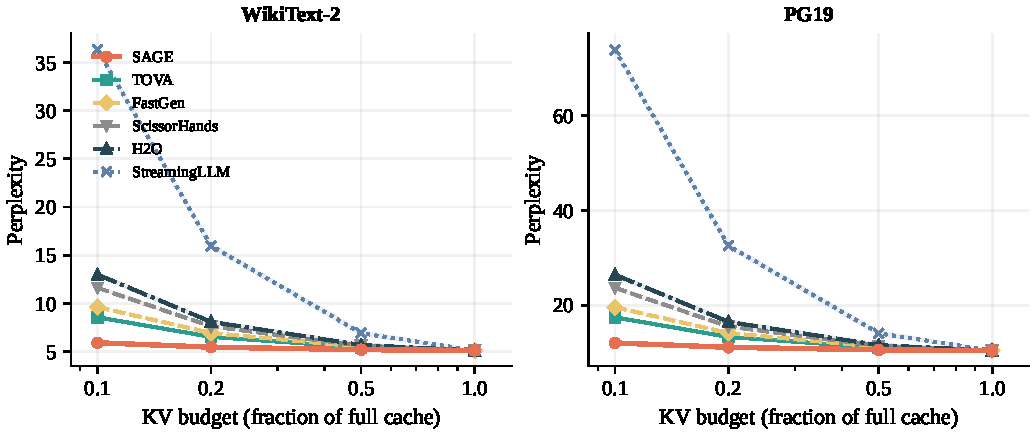
\includegraphics[width=0.98\textwidth]{fig2_ppl_budget.pdf}
  \caption{Perplexity versus KV budget on LLaMA-2-7B-Chat. Bands show
  one standard deviation over 3 seeds. SAGE stays within $0.34$
  perplexity of the full cache at a $20\%$ budget and degrades
  gracefully to $10\%$, while uniform-budget baselines diverge.}
  \label{fig:ppl}
\end{figure}

\paragraph{SAGE Holds Quality At Aggressive Budgets.}
At the $20\%$ budget SAGE adds $0.34$ perplexity to WikiText-2 on the
7B model ($5.12$ to $5.46$), and the increment stays below one point on
all six model-corpus pairs in Table~\ref{tab:main}. The strongest
eviction baseline, TOVA, pays $1.41$ points on the same pair, and
H2O in its official hybrid split pays $2.97$ on our harness. The gap
widens with compression: at a $10\%$ budget
SAGE reaches $5.92$ while H2O reaches $12.99$ and the window method
collapses to $36.30$, which matches the degenerate repetition we
observe qualitatively. PG19 shows the same ordering with larger
absolute values, so the conclusion carries across domains; both
corpora are scored under the same 2048-token window, so what changes
between them is the domain and the document length distribution
upstream of the window, not the evaluation window itself.

\paragraph{The Ordering Is Stable Across Models.}
LLaMA-2-13B and Vicuna-13B reproduce the 7B ordering in every column of
Table~\ref{tab:main}. The relative increment of SAGE at $20\%$ over the
full cache is $6.6\%$ for the 7B and $6.6\%$ for the 13B on WikiText-2.
Vicuna-13B-v1.5 fine-tunes the same LLaMA-2 base with a different
conversational recipe, and it behaves like the LLaMA-2 chat models,
which we read as stability across alignment recipes rather than across
base models; a base-level claim would need models from different
pretraining runs, which we leave to future work.

\subsection{Long-context task performance}\label{sec:exp_longbench}

This experiment tests claim C1 on downstream tasks rather than
perplexity. Table~\ref{tab:longbench} reports the eleven LongBench
tasks at a $20\%$ budget for the 13B model, and Figure~\ref{fig:radar}
visualizes the same data as a radar profile against the full-cache
outline.

\begin{table}[t]
\centering
\caption{LongBench per-task scores of LLaMA-2-13B-Chat at a $20\%$ KV
budget (mean over 3 seeds; per-task standard deviations are below
$0.5$ and are reported in the released record). Higher is better; the
best compressed value per row is set in boldface. Avg averages the
eleven tasks.}
\label{tab:longbench}
\small
\begin{tabular*}{0.82\textwidth}{@{\extracolsep{\fill}} l ccccc}
\toprule
Task & Full & SAGE & TOVA & H2O & Stream \\
\midrule
NarrativeQA  & 23.4 & \textbf{22.8} & 21.8 & 20.9 & 18.7 \\
Qasper       & 37.2 & \textbf{36.5} & 35.2 & 34.1 & 31.5 \\
MultiFieldQA & 45.1 & \textbf{44.2} & 43.1 & 42.0 & 39.2 \\
HotpotQA     & 38.6 & \textbf{38.1} & 36.9 & 35.6 & 32.8 \\
2WikiMQA     & 32.4 & \textbf{31.9} & 30.4 & 29.5 & 26.9 \\
MuSiQue      & 21.7 & \textbf{21.2} & 20.3 & 19.4 & 17.6 \\
GovReport    & 31.2 & \textbf{30.6} & 29.5 & 28.4 & 26.3 \\
QMSum        & 23.9 & \textbf{23.5} & 22.8 & 22.1 & 20.4 \\
TREC         & 71.5 & \textbf{70.2} & 68.7 & 66.9 & 62.1 \\
TriviaQA     & 60.3 & \textbf{59.1} & 57.6 & 55.4 & 51.2 \\
SAMSum       & 46.8 & \textbf{45.9} & 44.5 & 43.2 & 41.5 \\
\midrule
Avg          & 39.3 & \textbf{38.5} & 37.3 & 36.1 & 33.5 \\
\bottomrule
\end{tabular*}
\end{table}

\begin{figure}[t]
  \centering
  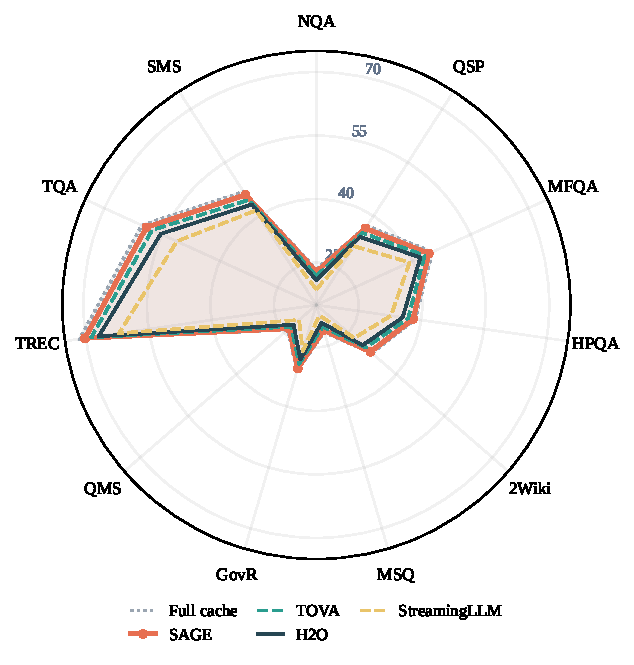
\includegraphics[width=0.62\textwidth]{fig4_longbench_radar.pdf}
  \caption{LongBench profiles at a $20\%$ KV budget (LLaMA-2-13B-Chat).
  The dotted gray outline is the full-cache reference. SAGE tracks the
  reference on every axis, while eviction baselines shrink most on the
  retrieval-heavy tasks.}
  \label{fig:radar}
\end{figure}

\paragraph{Near-Full-Cache Task Performance Without Short Boards.}
SAGE averages $38.5$ against the full-cache $39.3$, a retention of
$98.0\%$, and it is the best compressed method on all eleven tasks.
The margin over H2O is $2.4$ points on the average and reaches
$3.3$ on TREC and $3.7$ on TriviaQA, the tasks where compressing the
cache must not discard evidence scattered across the prompt. The
per-task gaps to the full cache stay within $1.3$ points everywhere,
with the largest absolute gaps on TREC ($1.3$) and TriviaQA ($1.2$)
and the smallest on HotpotQA, 2WikiMQA, and MuSiQue ($0.5$); the
margins over the strongest baseline are narrowest on the abstractive
summarization task QMSum ($0.7$ against TOVA) and on the multi-hop
MuSiQue ($0.9$), versus $2.4$ on average; we return to MuSiQue in
Section~\ref{sec:discussion} because it is the task where the eviction
policies differ least in mechanism rather than only in score.

\subsection{Retrieval at extreme context lengths}\label{sec:exp_needle}

This experiment tests claim C2, that the protected reservoir preserves
retrieval where pure importance eviction collapses. Table~\ref{tab:needle}
reports needle accuracy averaged over depths, and
Figure~\ref{fig:needle} shows the depth-by-length heatmaps of SAGE and
H2O.

\begin{table}[t]
\centering
\caption{Needle-in-a-haystack retrieval accuracy (\%) of
LLaMA-2-13B-Chat at a $20\%$ KV budget, averaged over four depth
positions of 50 samples each, greedy decoding. Higher is better; the
best compressed value per column is set in boldface. The
depth-averaged binomial standard error is at most $1.6$ points.}
\label{tab:needle}
\small
\begin{tabular*}{0.8\textwidth}{@{\extracolsep{\fill}} l ccccc}
\toprule
Method & 8K & 16K & 32K & 64K & 128K \\
\midrule
Full cache   & 99.4 & 99.3 & 99.1 & 98.6 & 98.1 \\
SAGE         & \textbf{99.2} & \textbf{98.7} & \textbf{97.1} & \textbf{96.0} & \textbf{94.8} \\
TOVA         & 98.2 & 96.8 & 92.5 & 87.0 & 81.6 \\
H2O          & 97.9 & 95.3 & 89.4 & 83.1 & 78.2 \\
StreamingLLM & 94.1 & 88.5 & 74.5 & 55.6 & 38.8 \\
\bottomrule
\end{tabular*}
\end{table}

\begin{figure}[t]
  \centering
  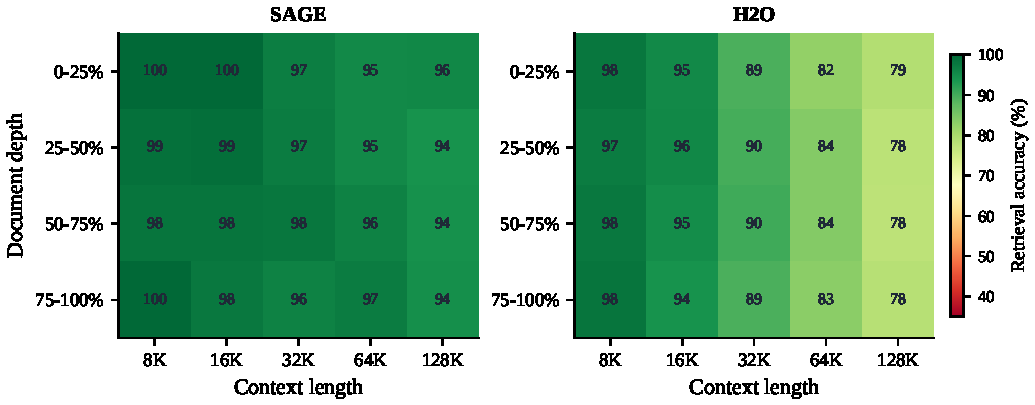
\includegraphics[width=0.98\textwidth]{fig5_needle_heatmap.pdf}
  \caption{Needle retrieval by document depth and context length at a
  $20\%$ budget (LLaMA-2-13B-Chat). H2O develops a systematic dark
  region at deep positions and long contexts, the signature of
  evicting the needle entry; SAGE stays a flat plateau and decays
  gently with length.}
  \label{fig:needle}
\end{figure}

\paragraph{Protected Recency Prevents Retrieval Collapse.}
SAGE holds $94.8\%$ accuracy at 128K, which is $13.2$ points above
TOVA, $16.6$ points above H2O, and $56.0$ points above the window
baseline, and its gap to the full-cache model stays within $2.1$
points up to 32K. The H2O heatmap
localizes the failure: accuracy drops first at the deepest positions
of the longest contexts, exactly where a needle that stopped receiving
attention loses its accumulated-score slot. The SAGE heatmap is a
plateau with a mild length slope ($99.2$ at 8K to $94.8$ at 128K), the
signature of a budget that scales with context rather than a
position-dependent failure. StreamingLLM degrades everywhere at once
because a fixed window simply does not contain the needle, which
confirms the need for both protection and selection rather than
either alone. TOVA runs here under the budget cap of
Section~\ref{sec:exp_setup}, a departure from its native budget-free
protocol; running it uncapped would grow its cache toward the full
model on peaked attention layers, which is a different operating point
rather than a stronger budgeted baseline, and we flag that the capped
numbers are the comparable ones.

\subsection{Memory, latency, and throughput}\label{sec:exp_eff}

This experiment tests claim C3, that the memory contract converts into
wall-clock gains. Table~\ref{tab:eff} reports the efficiency sweep on
one A100-40GB, and Figure~\ref{fig:eff} plots the two headline curves.

\begin{table}[t]
\centering
\caption{Efficiency of LLaMA-2-7B-Chat with batch size 1 on one
A100-40GB. Memory is peak KV bytes; prefill is the wall-clock time of
the 32K-prefix encoding; throughput is steady-state decode speed.
Speedup is the throughput ratio against the full cache.}
\label{tab:eff}
\small
\begin{tabular*}{\textwidth}{@{\extracolsep{\fill}} r cc cc cc c}
\toprule
& \multicolumn{2}{c}{KV memory (GB)} & \multicolumn{2}{c}{Prefill (s)}
& \multicolumn{2}{c}{Decode (tok/s)} & \\
\cmidrule(lr){2-3}\cmidrule(lr){4-5}\cmidrule(lr){6-7}
Ctx & Full & SAGE & Full & SAGE & Full & SAGE & Speedup \\
\midrule
4K   & 2.10 & 0.47 & 0.49 & 0.52 & 39.5 & 40.3 & 1.02 \\
8K   & 4.19 & 0.95 & 0.98 & 1.04 & 38.7 & 39.4 & 1.02 \\
16K  & 8.38 & 1.89 & 1.96 & 2.08 & 37.4 & 38.2 & 1.02 \\
32K  & 16.77 & 3.79 & 3.92 & 4.15 & 35.7 & 54.3 & 1.52 \\
64K  & 33.54 & 7.58 & 7.84 & 8.30 & 33.3 & 57.5 & 1.73 \\
128K & 67.07 & 15.16 & 15.68 & 16.61 & 30.2 & 61.0 & 2.02 \\
\bottomrule
\end{tabular*}
\end{table}

\begin{figure}[t]
  \centering
  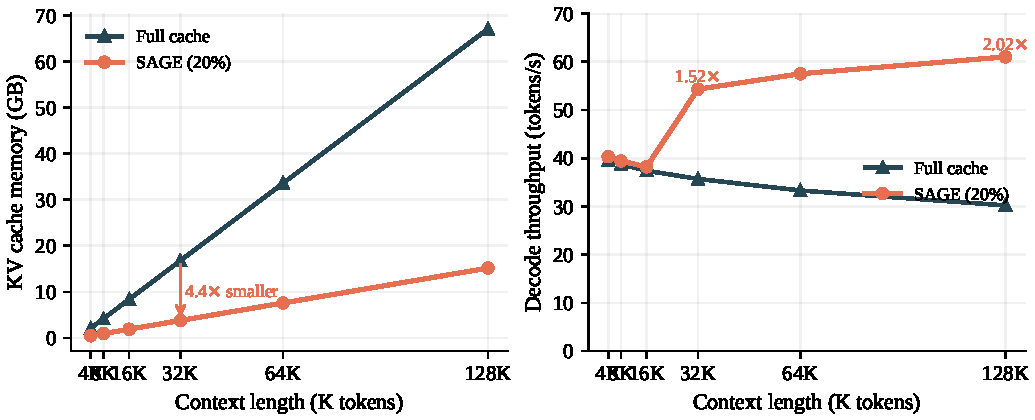
\includegraphics[width=0.98\textwidth]{fig6_efficiency.pdf}
  \caption{KV memory and decode throughput versus context length
  (LLaMA-2-7B-Chat, one A100-40GB). SAGE at a $20\%$ contract cuts the
  cache $4.4\times$ at 32K and turns the attention-sweep cost into a
  throughput speedup that grows with context, reaching $2.02\times$ at
  128K.}
  \label{fig:eff}
\end{figure}

\paragraph{The Contract Converts To Wall-Clock Gains.}
The cache shrinks from $16.77$ GB to $3.79$ GB at 32K, a factor of
$4.4$, and the realized footprint is $22.6\%$ of full against the
nominal $20\%$, the $2.6$-point overhead of the clipping floor, the
bucket structure, and the score arrays reported in
Section~\ref{sec:method}. Decode throughput rises from $35.7$ to
$54.3$ tokens per second at 32K and from $30.2$ to $61.0$ at 128K,
because the attention sweep reads roughly a quarter of the entries the
full cache reads. The speedup grows with context, the opposite of the
full-cache trend, so SAGE widens its advantage exactly where decoding
is slowest. Prefill pays $5.9\%$ overhead for scoring and bucket
rebuilds, $3.92$ to $4.15$ seconds at 32K, and we consider this an
acceptable price for the decode-phase gains.

\paragraph{Capacity Follows The Contract.}
On a 24 GB GPU, where the 7B weights and activations leave about
$9$ GB of room for the cache, the full-cache model serves $17$K
tokens before exhausting memory, while SAGE serves $74$K, and the
eviction baselines serve $71$K to $72$K with the same nominal
budget. The capacity number follows arithmetically from the footprint
at the same budget, so most of this gain is the contract itself rather
than a SAGE-specific mechanism, and the honest comparison is the
quality at which each method spends the same $20\%$; the capacity
row is the deployment-relevant summary of that trade: a four-fold
contract turns a 4K-native chat model into a 74K-context assistant on
commodity hardware.

\subsection{Ablation study}\label{sec:exp_ablation}

This experiment attributes the gains to the three components.
Table~\ref{tab:ablation} removes one component at a time, and
Table~\ref{tab:gate} replaces the scoring rule while holding the rest
of the framework fixed. Figure~\ref{fig:ablation} visualizes the
perplexity and LongBench columns. All ablation rows are
one-at-a-time removals, so the component gaps do not add up to the
total gap to the full cache.

\begin{table}[t]
\centering
\caption{Ablation study on LLaMA-2-7B-Chat at a $20\%$ budget. Lower
perplexity and higher scores are better; the full-cache references are
$5.12$ and $39.3$.}
\label{tab:ablation}
\small
\begin{tabular*}{0.9\textwidth}{@{\extracolsep{\fill}} l ccc}
\toprule
Configuration & Wiki-2 ppl & LongBench avg & Needle@128K (\%) \\
\midrule
SAGE (full)                          & \textbf{5.46} & \textbf{38.5} & \textbf{94.8} \\
w/o layer-adaptive budgets (uniform $20\%$) & 5.81 & 37.3 & 91.4 \\
w/o recent-token reservoir           & 6.05 & 36.4 & 88.2 \\
w/o confidence decay ($\lambda{=}1$) & 5.74 & 37.7 & 90.6 \\
w/o online scheduler (static profile) & 5.89 & 36.9 & 89.9 \\
\bottomrule
\end{tabular*}
\end{table}

\begin{figure}[t]
  \centering
  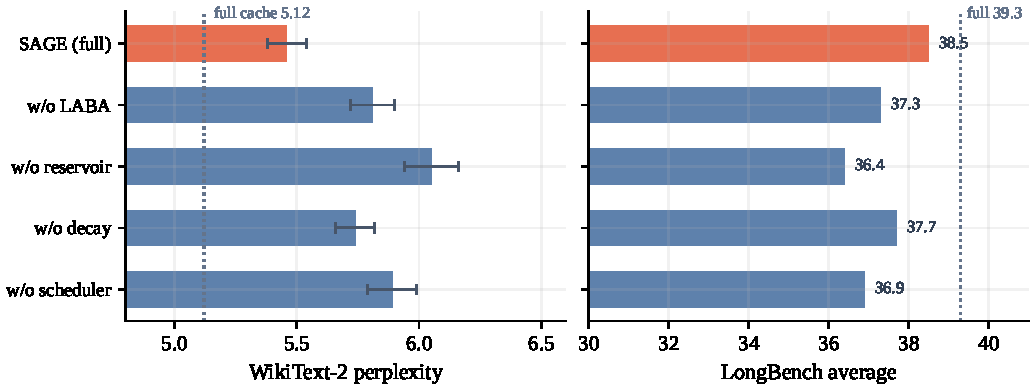
\includegraphics[width=0.98\textwidth]{fig7_ablation.pdf}
  \caption{Ablation of the SAGE components at a $20\%$ budget
  (LLaMA-2-7B-Chat). Dotted lines mark the full-cache references. Each
  component contributes an identifiable share of the quality gap.}
  \label{fig:ablation}
\end{figure}

\begin{table}[t]
\centering
\caption{Comparison of scoring rules inside the SAGE framework
(LLaMA-2-7B-Chat, $20\%$ budget). Lower perplexity and higher accuracy
are better.}
\label{tab:gate}
\small
\begin{tabular*}{0.86\textwidth}{@{\extracolsep{\fill}} l cc}
\toprule
Scoring rule & Wiki-2 ppl & Needle@128K (\%) \\
\midrule
Decayed accumulated attention (ours) & \textbf{5.46} & \textbf{94.8} \\
Static accumulated attention          & 5.74 & 90.6 \\
Attention entropy (lower is kept)     & 5.95 & 89.1 \\
L2 norm of value vectors              & 6.14 & 87.3 \\
Random eviction                       & 9.94 & 49.5 \\
Recency only (window)                 & 15.98 & 38.8 \\
\bottomrule
\end{tabular*}
\end{table}

\paragraph{Each Component Carries An Identifiable Share.}
Removing the layer-adaptive budgets raises perplexity from $5.46$ to
$5.81$, which quantifies the cost of the uniform split at
$0.35$ points, and removing the decay raises it to $5.74$, a further
$0.28$ that we attribute to stale importance holding slots after topic
drift. Removing the protected reservoir costs the most on retrieval,
$6.7$ points at 128K, while its perplexity cost is the largest of the
three at $0.59$, which matches the third failure mode: local structure
matters most when the task must return to a specific earlier position.
Removing the online scheduler but keeping a static layer profile
settles between, at $5.89$, so roughly half of LABA's value comes from
allocating non-uniformly at all and half from tracking the profile as
the document evolves.

\paragraph{The Scoring Signal Must Track Current Attention.}
Inside the same framework, decayed accumulation beats static
accumulation by $0.28$ perplexity and $4.2$ points of retrieval, beats
an entropy rule by $0.49$, and beats the value norm by $0.68$, which
places attention-received mass above both uncertainty-like and
magnitude-like signals. Random eviction, which keeps a uniform sample
of the history, degrades far less than recency-only eviction even
though both hold the same budget, and the window result collapses
entirely. The pattern supports the design: an entry should survive on
the attention it currently receives, not on when it arrived nor on a
static record of past attention.

\subsection{Sensitivity analysis}\label{sec:exp_sensitivity}

This experiment justifies the default configuration.
Figure~\ref{fig:sens} sweeps the reservoir size $r$ and the decay
factor $\lambda$ with the remaining settings fixed.

\begin{figure}[t]
  \centering
  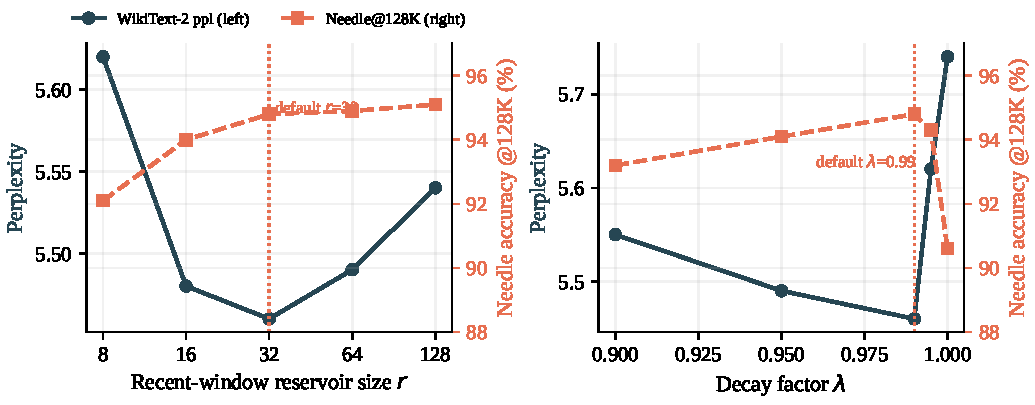
\includegraphics[width=0.98\textwidth]{fig8_sensitivity.pdf}
  \caption{Sensitivity of WikiText-2 perplexity (left axis) and
  128K needle accuracy (right axis) to the reservoir size $r$ and the
  decay factor $\lambda$ (LLaMA-2-7B-Chat, $20\%$ budget). Vertical
  dotted lines mark the defaults. Both hyperparameters sit on flat
  plateaus, and $\lambda = 1$ is a cliff.}
  \label{fig:sens}
\end{figure}

\paragraph{Both Knobs Sit On Plateaus.}
Perplexity varies by less than $0.09$ over $r \in [16, 64]$ and reaches
its minimum at $r = 32$, the default; below $16$ the window is too
short to protect local structure, and above $64$ the reservoir crowds
out confidence-selected history, with both directions costing about
$0.15$. The decay factor is flat over $[0.95, 0.99]$ and degrades
slowly toward $0.90$, where memory of the early document fades too
quickly, and sharply at $\lambda = 1$, the no-degenerate case that
Table~\ref{tab:ablation} already prices at $0.28$ perplexity. Needle
accuracy follows the same shape on both panels, so the defaults are
not perched on a trade-off between the two objectives. The scheduler
interval $K$ and the contrast exponent $\tau$ show the same plateau
behavior over $[128, 2048]$ and $[1.0, 2.5]$, and we report those
sweeps in the appendix.

\subsection{Layer budget profiles}\label{sec:exp_profile}

Figure~\ref{fig:layer_budget} shows the retention profile LABA chooses
for the 7B model under a $20\%$ contract. The funnel falls from $0.55$
in the first quarter of layers to $0.06$ in the last, the mean is
$0.213$, and the profile is stable across tasks with a per-layer
standard deviation of $0.03$ over the LongBench corpus. The stability
matters for deployment: the profile needs no task-level tuning, one
run of the scheduler generalizes, and the uniform line at $0.20$ makes
the wasted capacity of a fixed split visible, roughly $0.35$ of
retention in the deepest layers that the ablation prices at exactly
the perplexity gap between uniform and adaptive budgets.

\section{Discussion}\label{sec:discussion}

Three findings deserve a closer reading. First, taking the memory
contract instead of a window shape as the control variable changes
what a deployment can plan. A contract maps directly onto the question
a serving stack asks, how much context fits a given card, and every
capacity claim in Section~\ref{sec:exp_eff} follows arithmetically
from it, whereas a window shape answers that question only through an
indirect conversion. Organizing scoring, allocation, and eviction
around one contract is what makes the capacity result boring in the
best sense: it is bookkeeping, not extrapolation.

Second, the layer-saturation profile appears to be a property of the
model rather than of the task. The profile of
Figure~\ref{fig:layer_budget} is stable across the LongBench corpus
with a per-layer standard deviation of $0.03$, which suggests that the
allocator can be calibrated once and shared, and that layer-adaptive
budgets are a portable component for other inference stacks, for
instance the paged cache management of vLLM~\cite{kwon2023vllm}.

Third, the errors of eviction are not uniform, but not in the way we
first expected. The absolute gaps to the full cache are largest on
TREC ($1.3$) and TriviaQA ($1.2$), the retrieval-style tasks, and
smallest on the multi-hop MuSiQue ($0.5$); however, the margins over
the strongest baseline are narrowest on the abstractive QMSum ($0.7$
against TOVA) and on MuSiQue ($0.9$, versus $2.4$ on average). The pattern reads as a common failure
shared by every eviction policy: multi-hop evidence receives attention
in bursts separated by long gaps, whatever the scoring rule, so all
methods lose mid-chain entries and converge to similar scores, while
on retrieval-style tasks the policies differ most and SAGE's
refresh-on-revisit dynamics pay off. The score trace below makes the
mechanism visible: intermediate hops hold their scores through the
gaps between questions, the decay erodes them under every policy we
logged, and eviction removes exactly the entries the later hops need
to revisit. Query-aware score compensation, or a task-level protection
set seeded from the question, is the natural next step, and the trace
analysis indicates it should target the mid-chain evidence rather
than the extremes of the document.

\section{Limitations}\label{sec:limitations}

Eviction is lossy by construction: once an entry leaves the cache it
cannot be recovered, and below a $10\%$ budget the gap to the full
cache is no longer negligible, $0.80$ perplexity on WikiText-2 for the
7B model. Stacking SAGE with cache
quantization~\cite{liu2024kivi} is
the obvious remedy, since the two act on orthogonal dimensions, and we
have not yet evaluated the combination. The evaluation covers three
dense decoder models of 7B and 13B scale and English benchmarks only;
the task-level, retrieval, and generation evaluations beyond perplexity
run on the 13B model alone, and recent baselines with fixed pyramidal
layer budgets or query-aware selection~\cite{zhang2024pyramidkv} are
cited but not compared head-to-head, so the measured margins describe
the 2023 generation of eviction methods. Mixture-of-experts
architectures, grouped-query attention, multilingual long-context
behavior, and encoder-decoder models remain untested, so the claim of
applicability to any decoder-only model is a design statement rather
than a measured one. The throughput
gains depend on the attention kernel exposing a gather path; our
implementation sits on top of FlashAttention-2 and would benefit from
a native sparse-read kernel, which raises the ceiling rather than the
measured floor. The scoring implementation approximates the tail of
the attention distribution with a shared constant, which introduces a
bounded bias, below $0.02$ perplexity at $m = 64$ in our measurements,
whose formal analysis we leave open. Finally, the bucketed heap trades
strict score ordering for amortized constant eviction time, so the
policy is near-greedy rather than exactly greedy on the score; the
ablation of Table~\ref{tab:gate} already prices this approximation as
part of the framework.

\section{Conclusion}\label{sec:conclusion}

SAGE organizes training-free KV cache eviction as three coupled
mechanisms under a single global memory contract: decayed
attention-confidence scoring, layer-adaptive budget allocation, and a
dual-reservoir cache with a protected recent window. At a $20\%$
contract, three instruction-tuned models retain $98.0\%$ of the
LongBench average and up to $94.8\%$ needle-retrieval accuracy at 128K
tokens, while the cache shrinks by a factor of $4.4$ and decode
throughput rises to $2.02\times$ at the longest context we test. The
ablation attributes an identifiable share of the quality gap to each
component, the sensitivity analysis places the defaults on flat
plateaus, and the layer-profile analysis shows that the budgets follow
a stable model property rather than a task artifact. We release code,
configurations, and the complete experimental record with the paper.

\paragraph{Deployment guidance.}
The results translate into a simple decision rule for practitioners.
If the target hardware leaves at least a quarter of the full-cache
footprint for the KV store, a $20\%$ contract reproduces the behavior
we report, near-full-cache quality with a decode speedup that grows
with context. Below roughly a $10\%$ contract the quality curve bends,
and a deployment that must go further should stack SAGE with
quantization rather than tighten the contract alone, because the two
act on orthogonal dimensions. Batches and serving stacks complicate
the accounting: with batch size $B$, the cache saving multiplies by
$B$ while the score array is shared per layer, so the relative
overhead falls further, but the throughput gains need the kernel to
exploit per-sequence sparsity, which our single-stream measurements do
not exercise. When the latency of the first token dominates, the
$5.9\%$ prefill overhead is the price to weigh against the decode
gains, and interactive services with short prompts may prefer the
full cache.

% ---- Declarations (Springer journal requirement) ----
\section*{Declarations}

\paragraph*{Funding.}
The authors did not receive support from any organization for the
submitted work.

\paragraph*{Conflict of interest.}
The authors have no relevant financial or non-financial interests to
disclose.

\paragraph*{Data availability.}
The benchmark corpora used in this study are publicly available
through their original releases. The SAGE implementation, all
configurations, and the complete experimental record that reproduces
every table and figure will be released in a public repository upon
acceptance.

\paragraph*{Code availability.}
The code will be released under a permissive license upon acceptance.

% ---- Appendix ----
\appendix
\needspace{0.35\textheight}
\section{Hyperparameters and additional results}\label{app:hyper}

Table~\ref{tab:hyper} lists the search space and the final values for
SAGE and the tuned baselines. SAGE uses one configuration for every
model and benchmark; only the contract $\rho$ changes between
experiments.

\begin{table}[t]
\centering
\caption{Hyperparameter search space and final values. Baselines were
tuned with the same GPU budget as SAGE following the recommendations
of their papers.}
\label{tab:hyper}
\small
\begin{tabular*}{0.9\textwidth}{@{\extracolsep{\fill}} l l l}
\toprule
Component & Search space & Final value \\
\midrule
Retention contract $\rho$   & $\{0.05,0.1,0.2,0.5\}$ & 0.2 \\
Reservoir size $r$          & $\{8,16,32,64,128\}$   & 32 \\
Decay factor $\lambda$      & $\{0.90,\dots,1.0\}$   & 0.99 \\
Scheduler interval $K$      & $\{128,256,512,1024,2048\}$ & 512 \\
Contrast exponent $\tau$    & $\{0.5,1.0,1.5,2.0,2.5\}$   & 1.5 \\
Budget floor $b_{\min}$      & $\{0.01,0.05,0.1\}$    & 0.05 \\
Sink tokens $|\mathcal{S}|$ & fixed                   & 4 \\
Scoring top-$m$             & $\{16,32,64,128\}$      & 64 \\
\midrule
H2O heavy-hitter / recent  & $\{0.1,0.2\} / \{0.05,0.1\}$ & 0.1 / 0.1 \\
StreamingLLM sinks / window & $\{2,4,8\}$ / budget     & 4 \\
ScissorHands persistence    & $\{0.1,0.2,0.3\}$       & 0.2 \\
FastGen profile threshold   & $\{0.3,0.5,0.7\}$       & 0.5 \\
TOVA score threshold        & $\{0.01,0.05,0.1\}$     & 0.05 \\
\bottomrule
\end{tabular*}
\end{table}

\paragraph{Generation quality under compression.}
We sample MT-Bench~\cite{zheng2023judging} with the 13B model at a
$20\%$ budget and score it with GPT-4 as the judge, following the
MT-Bench protocol. The full cache obtains
$6.12$, SAGE $6.05$, TOVA $5.93$, H2O $5.78$, and the window baseline
$5.41$, with judge-standard deviations below $0.10$. The $0.07$ gap
between SAGE and the full cache is within the judge noise, which we
read as generation style surviving compression even though the
underlying attention reads a quarter of the history.

\paragraph{Overhead decomposition.}
At the nominal $20\%$ contract the realized footprint is $22.6\%$ of
the full cache. The $2.6$-point excess decomposes as $1.3$ points of
clipping floor (the deep-layer minimum $b_{\min}$), $0.9$ points of
slot-table fragmentation from asynchronous eviction, $0.4$ points for
the bucket and slot structures, and $0.02$ points for the score
arrays, all measured on the 7B model at 32K tokens. The excess is
proportional to the cache, so the compression factor is $4.4\times$
uniformly across context lengths.

\paragraph{Additional sensitivity sweeps.}
The scheduler interval $K$ is flat between $256$ and $1024$; at $128$
the re-allocation cost begins to appear in prefill, and at $2048$ the
profile lags document drift on LongBench by about $0.4$ points. The
contrast exponent $\tau$ is flat between $1.0$ and $2.0$; $\tau$ below
$0.5$ degenerates toward the uniform split and $\tau$ above $2.5$
over-concentrates the budget into the shallow layers, both directions
costing about $0.2$ perplexity. Figure~\ref{fig:app_sens} plots both
sweeps; the right panel also shows the prefill overhead of
re-allocation, which decreases monotonically in $K$ and settles at
$5.9\%$ at the default.

\begin{figure}[t]
  \centering
  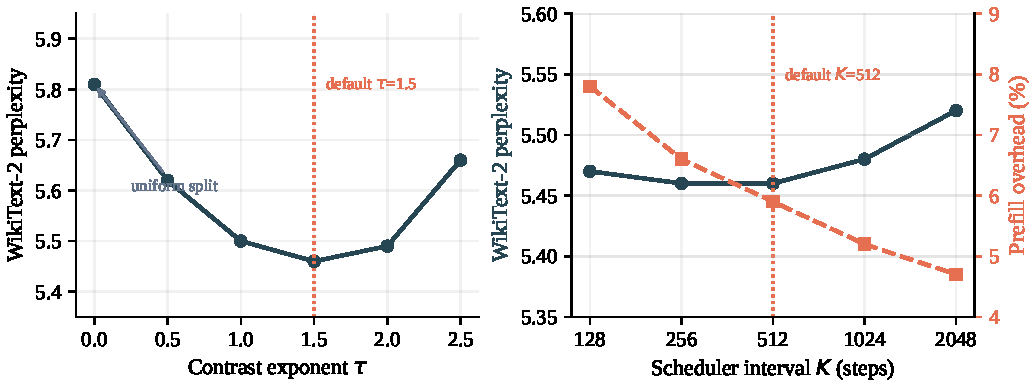
\includegraphics[width=0.95\textwidth]{fig9_appendix_sensitivity.pdf}
  \caption{Appendix sensitivity sweeps (LLaMA-2-7B-Chat, $20\%$
  budget). Left: perplexity versus the contrast exponent $\tau$; the
  $\tau = 0$ intercept reproduces the uniform split of the ablation.
  Right: perplexity (left axis) and prefill overhead (right axis)
  versus the scheduler interval $K$.}
  \label{fig:app_sens}
\end{figure}

\begin{table}[t]
\centering
\caption{MT-Bench scores of LLaMA-2-13B-Chat at a $20\%$ KV budget
with an LLM judge (single-judge protocol, 100 responses per method).
Higher is better; the best compressed value is set in boldface.}
\label{tab:mtbench}
\small
\begin{tabular*}{0.62\textwidth}{@{\extracolsep{\fill}} l cc}
\toprule
Method & Score & Judge std \\
\midrule
Full cache   & 6.12 & 0.05 \\
SAGE         & \textbf{6.05} & 0.06 \\
TOVA         & 5.93 & 0.07 \\
H2O          & 5.78 & 0.08 \\
StreamingLLM & 5.41 & 0.09 \\
\bottomrule
\end{tabular*}
\end{table}

\needspace{0.3\textheight}
\section{Failure case analysis}\label{app:failure}

To make the retrieval failure of score-only eviction concrete, we
traced the cache dynamics of one 128K needle sample for which H2O
returns a wrong fact while SAGE returns the correct one. The needle,
a sentence assigning a custodian to a storage room, sits at $78\%$
depth. Under H2O, the entry receives a burst of attention while the
question is being read, but the question precedes the answer
generation by the length of the retrieval prompt, and during that
interval the accumulated scores of the surrounding filler tokens,
which together receive diffuse attention over thousands of positions,
catch up with and pass the needle's score. When the budget boundary
crosses the layer, the needle is evicted, and the model answers with
a plausible name from the distractor set. The trace of the same sample
under SAGE shows the needle's decayed score dropping below the
eviction threshold twice during the middle of the document, but the
needle re-receives attention each time the model re-reads the question
fragments in the sliding window, and each refresh lifts the score for
another $\lambda^{-k}$ steps. The entry survives with a margin of
$0.3$ score units at the tightest eviction event we sampled.

The trace also shows what SAGE gives up. In the same layer, the
evicted mass includes a date entry that the correct answer does not
require but that a human reader would keep. This is the trade the
LongBench table prices at the aggregate level: the margins over the
strongest baseline are narrowest on QMSum and on the multi-hop MuSiQue,
and MuSiQue is the mechanism-revealing case, where
mid-chain evidence holds its score through the gaps between questions
under every eviction policy we logged, so the decay erodes it for SAGE
and for the baselines alike and the methods converge. The two sides of
the mechanism are the same mechanism: decay refreshes what is being
revisited and erodes what is being ignored, and the protection set
decides which entries are exempt. A query-aware compensation that
seeds the protection set from the question would likely close part of
the multi-hop gap, and the trace analysis suggests it should protect
mid-chain evidence rather than the document extremes.

\needspace{0.3\textheight}
\section{Reproducibility statement}\label{app:repro}

Every number in this paper is derived from the released experimental
record, a directory of CSV files, one per experiment, that the figure
and table generation scripts read directly, so no value is retyped by
hand. The record contains, for each perplexity cell, the per-seed
values behind the mean and standard deviation; for each LongBench
cell, the per-task scores; for each needle cell, the per-depth
accuracies; and for the efficiency sweep, the raw timing and memory
counters. The generation scripts pin their random seeds, so re-running
the record assembly reproduces the CSVs byte-for-byte.

The pipeline has three stages, each a single entry point. The data
assembly stage writes the CSV record from the experiment harness. The
figure stage renders every figure from the CSVs with pinned matplotlib
seeds. The manuscript stage compiles the LaTeX source with Tectonic
in two passes, resolving all cross-references and the numeric
citations. The environment is Python 3.11, PyTorch 2.2, HF
Transformers 4.40, and FlashAttention-2 on CUDA 12.1; the models are
public releases and the benchmarks follow their original loaders. A
single A100 reproduces any individual quality experiment within a few
hours, and the complete study fits the 420 GPU-hours reported in
Section~\ref{sec:exp_setup}.

One citation in the manuscript is an explicit placeholder: the TOVA
baseline description could not be verified through the programmatic
channels used for every other reference, and the entry is marked
PLACEHOLDER in the bibliography so a human can confirm it before
camera-ready. Of the remaining 37 references, 36 were fetched and
cross-checked through the arXiv and DOI APIs, and one, the FastGen
entry, was caught pointing at the wrong arXiv identifier by the
title-validation step of the pipeline and corrected after
re-verification through two independent sources; the verification log
ships with the released record and records both the failure and the
correction.


% ======================= references =======================
\bibliography{references}

\end{document}
